\chapter{Metodologia}\label{metodologia}

\section{Ferramentas e Dados}\label{ferramentas-e-dados}

\subsection{Linguagem R}\label{linguagem-r}

R é uma linguagem e ambiente multiplataforma para análise estatística
com ferramentas gráficas avançadas. A linguagem implementa o paradigma
da programação funcional, bem como o da orientação a objetos. O projeto
R é distribuído sob a \sigla{GPL}{Licença Pública Geral} do projeto GNU \cite{rlang}. O GNU foi criado como uma reação aos \emph{softwares} proprietários
e de código fonte fechado, marcando o início do movimento do
\emph{software} livre, ou seja, programas de computador com código fonte
aberto e que está disponível para que qualquer um o estude, copie,
modifique e o redistribua.\cite{torres2013tecnoutopia}

\subsubsection{Ambiente R}\label{ambiente-r}

O desenvolvimento e crescimento da comunidade em torno do R se deu
pela sua capacidade de integração com outros \emph{softwares},
facilitando assim, por exemplo, a integração com diversas bibliotecas
SIG. O uso da linguagem torna-se mais amigável com o Ambiente de
Desenvolvimento Integrado (\emph{IDE}) chamado \emph{Rstudio}, que
possui recursos como painéis de visualização interativos, acesso a
documentação dos pacotes diretamente pela linha de comando ou painel,
criação e manutenção de projetos, entre outros. \cite{geocompr}

Através da linha de comando, é muito simples instalar um pacote ou
então acessar sua documentação, que é um dos pontos fortes do R. Todos
os pacotes estão armazenados em uma rede de servidores chamada CRAN, ou
\emph{Comprehensive R Archive Network}, onde a comunidade desenvolvedora
mantém um padrão de documentação muito bem organizado. Para que um
pacote esteja disponível no CRAN, é necessário por exemplo um manual com
referências teóricas para cada método implementado, e geralmente possuem
exemplos simples e intuitivos, que também podem ser acessados com
facilidade pela linha de comando.

\subsubsection{Rmarkdown}\label{rmarkdown}

\emph{Markdown} é uma linguagem marcação simples cujo texto é
convertido para o \sigla{HTML}{Linguagem de Marcação de Hipertexto}. O
\emph{RMarkdown} é uma adaptação do \emph{markdown} para o R que em
conjunto com outros pacotes, pode ser facilmente convertida para
formatos como \sigla{PDF}{\emph{Portable Document Format}}, arquivos de texto,
\acs{HTML}, apresentação de slides, entre outros. Sua importância está na
divulgação de resultados de análises que poderão ser facilmente
reproduzidas por outras pessoas.

Com o \emph{RMarkdown} é possível escrever texto no formato LaTeX,
adicionar trechos de código (\emph{chunks}) que por sua vez imprimirão
seu resultado, seja ele um gráfico, uma tabela ou texto. De maneira
integrada ao RStudio, os \emph{chunks} também possuem suporte a outras
linguagens como Python.

\subsubsection{Bibliotecas}\label{bibliotecas}

Para a realização deste trabalho, foram utilizadas, dentro do ambiente
de desenvolvimento RStudio, bibliotecas quem fazem a \emph{interface}
com a \acs{GDAL}, uma biblioteca
tradutora para dados geoespaciais \emph{raster} e vetoriais que é
utilizada por muitos \emph{software} de \acs{SIG}.

\subsection{Google Earth Engine}\label{google-earth-engine}

O \emph{Google Earth Engine} é uma plataforma de processamento
geoespacial baseada em nuvem, feito principalmente para análises de
dados ambientais em escala planetária. O acesso a plataforma foi
utilizado para a obtenção e processamento de dados de treinamento. \cite{gorelick2017google}

\subsection{Iniciativas}\label{iniciativas}

\subsubsection{Mapbiomas}\label{mapbiomas}

\begin{citacao}
O Projeto de Mapeamento Anual da Cobertura e Uso do Solo do Brasil é uma
iniciativa que envolve uma rede colaborativa com especialistas nos
biomas, usos da terra, sensoriamento remoto, SIG e ciência da computação
que utiliza processamento em nuvem e classificadores automatizados
desenvolvidos e operados a partir da plataforma Google Earth Engine para
gerar uma série histórica de mapas anuais de cobertura e uso da terra do
Brasil. \cite{mapbiomas2018coleccao}
\end{citacao} 

O MapBiomas é uma plataforma aberta e colaborativa com uma metodologia
de baixo custo que pode ser aplicada em diversos contextos. Grande parte
deste trabalho teve essa iniciativa como referência, e também, parte dos
dados que foram utilizados no modelo de classificação foram obtidos da
Coleção 3.1 do projeto \cite{mapbiomas2018coleccao}, através do próprio \emph{site} e também pela
plataforma do Google Earth Engine. Os detalhes estão explicados no próximo capítulo.

Além do mapeamento anual dos biomas brasileiros, também a outras
iniciativas como o MapBiomas Alerta:

\begin{citacao}
"MapBiomas Alerta é um sistema de validação e refinamento de alertas de
desmatamento, degradação e regeneração de vegetação nativa com imagens
de alta resolução." \cite{mapbiomas2018coleccao}
\end{citacao}

% \subsubsection{Outras iniciativas}\label{outras-iniciativas}

% Pensando em monitoramento do uso e cobertura da terra, por meio de
% análise de imagens de satélite num contexto Brasileiro, é importante
% destacar outras iniciativas.

% O Instituto do Homem e Meio Ambiente da Amazônia (IMAZON) é um
% instituto que possui o programa de Monitoramento da Amazônia tem por
% objetivo monitorar e detectar desmatamento, a exploração madeireira e
% outras formas de pressão humana.
% (https://imazon.org.br/programas/monitoramento-da-amazonia/)



% \begin{quote}
% O sistema PRODES do INPE fornece uma série histórica anual e
% ininterrupta do corte raso (áreas totalmente desmatadas) na Amazônia
% desde 1988, permitindo análises comparativas. Além disso, o INPE mantém
% desde 2004 o DETER, um sistema de apoio à fiscalização que produz
% diariamente alertas sobre corte raso e também de áreas em processo de
% degradação florestal (exploração de madeira, mineração, queimadas e
% outras). Esses alertas são enviados automaticamente ao Ibama, para o
% planejamento das ações de fiscalização. As informações ficam ainda
% disponíveis na internet para as Secretarias Estaduais de Meio Ambiente,
% bem como para toda a sociedade.
% (http://www.inpe.br/noticias/noticia.php?Cod\_Noticia=5179)
% \end{quote}

% \begin{quote}
% Em 2018, o INPE expandiu o monitoramento para o Cerrado. Somados aos
% dados produzidos para a Amazônia, o Instituto garante uma base de
% informações sobre o desmatamento em áreas de vegetação natural de 73\%
% do território brasileiro.

% A série histórica de dados orbitais sobre desmatamento norteia vários
% estudos científicos e políticas públicas, produzindo informação para
% toda a sociedade interessada em sustentabilidade. O INPE também monitora
% queimadas e a qualidade do ar, entre outros índices importantes na área
% de clima e meio ambiente.
% http://www.inpe.br/noticias/noticia.php?Cod\_Noticia=5124
% \end{quote}

\subsection{Satélites}\label{satuxe9lites}

Num contexto de Obervação da Terra (OT), a fim de monitorar os
recursos terrestres, há uma grande quantidade de programas de satélites
que orbitam o globo com a tarefa de fazer o imageamento da superfície
terrestre. 

O Instituto Nacional de Pesquisas Espaciais (INPE) possui um papel
fundamental e histórico para o uso de Sensorimento Remoto em escala nacional. Foi pioneiro no desenvolvimento e formação nas áreas de interpretação de imagens e processamento digital \cite{meneses2012introduccao}.

O instituto realiza a distribuição de imagens geradas por
diversos desses programas através da sessão de Divisão de Geração de
Imagens, como: o Landsat e TERRA, dos Estados Unidos; o
RESOURCESAT, da Índia; o RapidEye da Alemanhã; bem como o AQUA, uma parceria entre Brasil e Japão; e ainda o CBERS, parceria entre Brasil e China que tem como objetivo o monitoramento de biomas, agricultura,
crescimento urbano, gerenciamento hídrico e de desastres naturais. \cite{inpe-dgi}

Vale o destaque para o Landsat, programa de origem norte americana
gerenciado pela \sigla{NASA}{Administração Nacional da Aeronáutica e Espaço}  e
o \sigla{USGS}{Serviço Geológico dos Estados Unidos}, que realizou uma série de
lançamentos desde a década de 1970. Em um contexto, vindo da década
anterior, da corrida espacial e as primeiras imagens da Terra capturadas
por satélites, a história desse programa se confunde com o
desenvolvimento das técnicas de SR e interpretação de imagens digitais.
Também há o programa de Observação da Terra da União Europeia, o Copernicus, desenvolvido
em parceria com a \sigla{ESA}{Agência Espacial Europeia}, que possui a missão dos satélites Sentinel, com características semelhantes as do Landsat (ambos possuem resolução espacial média, por exemplo).

É importante destacar também o advento dos nano e microsatélites, que
geralmente carregam sensores com uma resolução espacial maior e menor
custo de lançamento, porém, com menor resolução radiométrica. Lembrando
que cada característica dos sensores possuem diferentes fins de
aplicações.

Os dados dos satélites do programa \emph{Landsat} e \emph{Sentinel}
possuem acesso aberto desde 2008 e 2013, respectivamente. Estes são
marcos importantes num contexto de Observação da Terra, gerando demanda para a computação em nuvem, que resolvem problema de processamento e
armazenamento, enquanto o usuário pode focar no desenvolvimento do
algoritmo. \cite{wulder2014satellites}

\section{Etapas}\label{etapas}

	De acordo com \cite{lu-weng}, o sucesso da classificação de dados de SR em
um mapa temático depende de fatores como: complexidade da área de
estudo, seleção dos dados, abordagens de processamento de imagens e
seleção de sistema de classificação apropriado. Com base nos artigos de
\cite{lu-weng} e \cite{maxwell}, foi elaborado o seguinte processo descrito no fluxograma a seguir.

\begin{figure}[htbp]
    \centering
    \caption{Fluxograma do processo de desenvolvimento em etapas} \label{fig-fluxograma}
    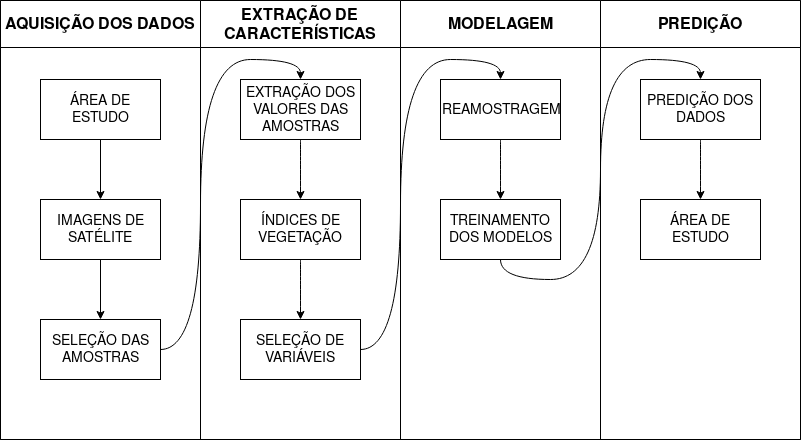
\includegraphics[scale=0.55]{figs/etapas.png}
    \legend{Fonte: Elaborado pelo autor}
\end{figure}
